\section{Arjun Yuda Firwanda}
\subsection{Soal 1}
Isi jawaban soal ke-1

Kalau mau dibikin paragrap \textbf{cukup enter aja}, tidak usah pakai \verb|par| dsb

%\subsection{Soal 2}
%Isi jawaban soal ke-2

%\subsection{Soal 3}
%Isi jawaban soal ke-3

\section{Dwi Yulianingsih}
\subsection{Soal 1}
\begin{enumerate}
\subsection{Soal 1}
 CSV (Comma Separated Value) adalah format basis data sederhana yang dimana setiap record yang ada dipisahkan dengan tanda koma (,) atau titik koma (;). Format data file csv dapat diolah dengan berbagai text editor dengan mudah. Anda tidak perlu (dan Anda tidak akan) membuat pengurai CSV Anda sendiri dari awal. Ada beberapa perpustakaan yang dapat diterima yang dapat Anda gunakan. Pustaka csv Python akan berfungsi untuk sebagian besar kasus. Jika pekerjaan Anda memerlukan banyak data atau analisis numerik, panda library juga memiliki kemampuan penguraian CSV, yang seharusnya menangani sisanya. Dalam bahasa pemrograman Python telah disediakan modul csv yang khusus untuk mengolah data berformat csv.  Untuk memanipulasi data csv dengan python tentunya yang pertama dilakukan adalah mengimport modul csv dengan perintah import csv. File CSV biasanya dibuat oleh program yang menangani sejumlah besar data. Mereka adalah cara yang nyaman untuk mengekspor data dari spreadsheet dan basis data serta mengimpor atau menggunakannya dalam program lain. Misalnya, Anda dapat mengekspor hasil program penambangan data ke file CSV dan kemudian mengimpornya ke dalam spreadsheet untuk menganalisis data, menghasilkan grafik untuk presentasi, atau menyiapkan laporan untuk publikasi. Contoh nya adalah sebagai berikut :

 \lstinputlisting[firstline=8, lastline=20]{src/4/1174009/dudul.py}

\subsection{Soal 2} 
 Ada beberapa aplikasi yang dapat menciptakan file dengan format csv diantaranya google sheet, number di MacOS dan microsoft excel.

\subsection{Soal 3}
 Cara membuat file csv di excel cukup mudah yaitu :
\begin{itemize}
	\item Buat foldernya
	\item Pilih save as
	\item pilih file dengan format csv
\end{itemize}
Cara membaca file di csv :
\begin{itemize}
	\item Klik data - get external data - form text
	\item Akan muncul Text Import Wizard, arahkan pada file csv yang ingin anda buka lalu Open.
	\item Setelah File terbuka, akan muncul Text Import Wizard.
	\item Pilih Delimited, Kemudian Next (Di sini, bisa juga menentukan baris awal yang akan di import)
	\item Centrang pada Tab dan Comma (Atau sesuai pengaturan File Anda) lalu Next.
	\item Atur Format data pada tiap kolom yang tampil dan klik Finish
\end{itemize}

\subsection{Soal 4}
 CSV muncul untuk memudahkan data science dan analis karena dinilai terdapat banyak kemudahan yang didapat. CSV dapat dimaksimalkan jika dipaduka dengan python karena python adalah bahasa pemrograman yang support ke banyak library termasuk csv. Maka karena itulah perpaduan python dan csv seringkali digunakan oleh perusahaan-perushaan besar dalam mengolah datanya.

\subsection{Soal 5}
Pandas merupakan tool yang dapat digunakan sebagai alat analisis data dan struktur untuk bahasa pemrograman Python. Pandas dapat mengolah data dengan mudah, salah satu fitur yang ada dalam pandas adalah Dataframe. Fitur dataframe dapat membaca sebuah file dan menjadikannya tabble, juga dapat mengolah suatu data dengan menggunakan operasi seperti join, group by dan teknik lainnya yang terdapat pada SQL. Dalam hal ini pandas tidak jauh beda dengan csv yaitu memiliki keunggulan dalam pengolahan data-data besar dan dapat disupport dengan baik dengan python walaupun mengimport data dalam jumlah banyak.

\subsection{Soal 6}
 Library csv mempunyai keunggulan dibandingkan format data lainnya adalah soal kompatibilitas. File csv dapat digunakan, diolah, diekspor/impor, dan dimodifikasi menggunakan berbagai macam perangkat lunak dan bahasa pemrograman. Pada library csv mempunyai fungsi import dan eksport data yang baik dan bisa digunakan dalam jumlah besar.

\subsection{Soal 7}
pandas menyediakan beragam fungsi operasi untuk mengolah data. Contoh jika menggunakan series bisa mencari nilai max, min, dan mean secara langsung, bahkan juga bisa melakukan operasi perpangkatan pada nilai Series secara langsung.
Pandas dapat mengolah suatu data dan mengolahnya seperti join, distinct, group by, agregasi, dan teknik seperti pada SQL. Hanya saja dilakukan pada tabel yang dimuat dari file ke RAM.
\end{enumerate}

\subsection{bukti bebas plagiarisme}
\begin{figure}[H]
\centering
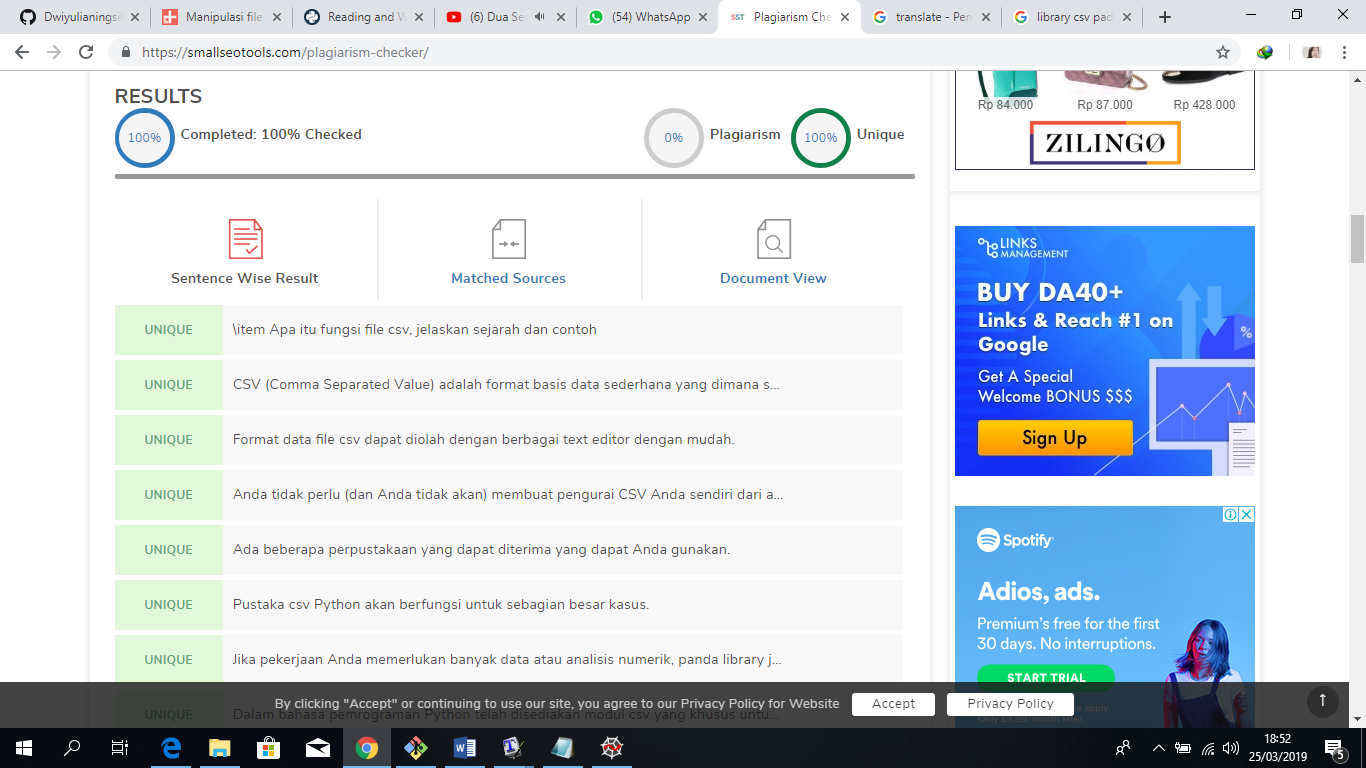
\includegraphics[width=10cm]{figures/4/1174009/yuli.png}
\caption{SS Bebas Plagiarisme}
\label{dwiyul}
\end{figure}


\section{Harun Ar-Rasyid}
\subsection{Soal 1}
File CSV (Nilai Terbatas Koma) adalah jenis file khusus yang dapat Anda buat atau edit di Excel. File CSV menyimpan informasi yang dipisahkan oleh koma, tidak menyimpan informasi dalam kolom. Ketika teks dan angka disimpan dalam file CSV, mudah untuk memindahkannya dari satu program ke program lainnya.
Dari rilis pertama, Excel menggunakan format file biner yang disebut Binary Interchange File Format (BIFF) sebagai format file utamanya. Ini berubah ketika Microsoft merilis Office System 2007 yang memperkenalkan Office Open XML sebagai format file utamanya. Office Open XML adalah file kontainer berbasis XML yang mirip dengan XML Spreadsheets (XMLSS), yang diperkenalkan di Excel 2002. File versi XML tidak bisa menyimpan makro VBA.
Meskipun mendukung format XML baru, Excel 2007 masih mendukung format lama yang masih berbasis BIFF tradisional. Selain itu Microsoft Excel juga mendukung format Comma Separated Values (CSV), DBase File (DBF), SYMbolic LinK (SYLK), Format Interchange Data (DIF) dan banyak format lainnya, termasuk format lembar kerja 1-2 Lotus - 3 (WKS, WK1, WK2, dll.) Dan Quattro Pro.

\subsection{Soal 2}
\begin{itemize}
    \item Texteditor
    Seperti notepad,visual studio code,atom,sublime dan lain sebagainya
    \item Program Spreadsheet
    Seperti excell,google spreadshare,LibreOfficecalc
\end{itemize}

\subsection{Soal 3}
Untuk menulisnya untuk yang paling atas itu kita buat headernya,untuk mepermudah membedakan datanya,dan untuk baris kedua dan seterusnya itu untuk data itu sendiri.
dan setelah di buat kalian save as kemudian pilih format CSV.
dan untuk membukan cukup di double clik file tersebut.

\subsection{Soal 4}
library csv dibuat untuk permudah mengolah data. Dan mempermudah untuk melakukan export dan import file csv itu sendiri

\subsection{Soal 5}
library pandas dibuat agar bahasa pemograman python bisa bersaing R dan matlab, yang digunakan untuk mengolah banyak data , keperluan big data, data mining data science dan sebagainya.

\subsection{Soal 6}
Terdapat 2 fungsi yang bisa digunakan oleh library csv
Pertama,fungsi membaca file csv.
fungsi ini bisa menggunakan list dan dictionary
Dengan list :
\lstinputlisting[firstline=11, lastline=21]{src/4/1174027/teori/c_1174027_csv.py}
Dengan dictionary :
\lstinputlisting[firstline=24, lastline=33]{src/4/1174027/teori/c_1174027_csv.py}
Kedua,fungsi menulis file csv.
\lstinputlisting[firstline=36, lastline=40]{src/4/1174027/teori/c_1174027_csv.py}

\subsection{Soal 7}
Hampir sama dengan library csv,tp library pandas penulisannya lebih sederhana dan terlihat lebih rapih dari pada library csv.
\lstinputlisting[firstline=10, lastline=11]{src/4/1174027/praktek/p_1174027_pandas.py}

\subsection{Bukti Bebas Plagiat}
\begin{figure}[H]
    \centering
    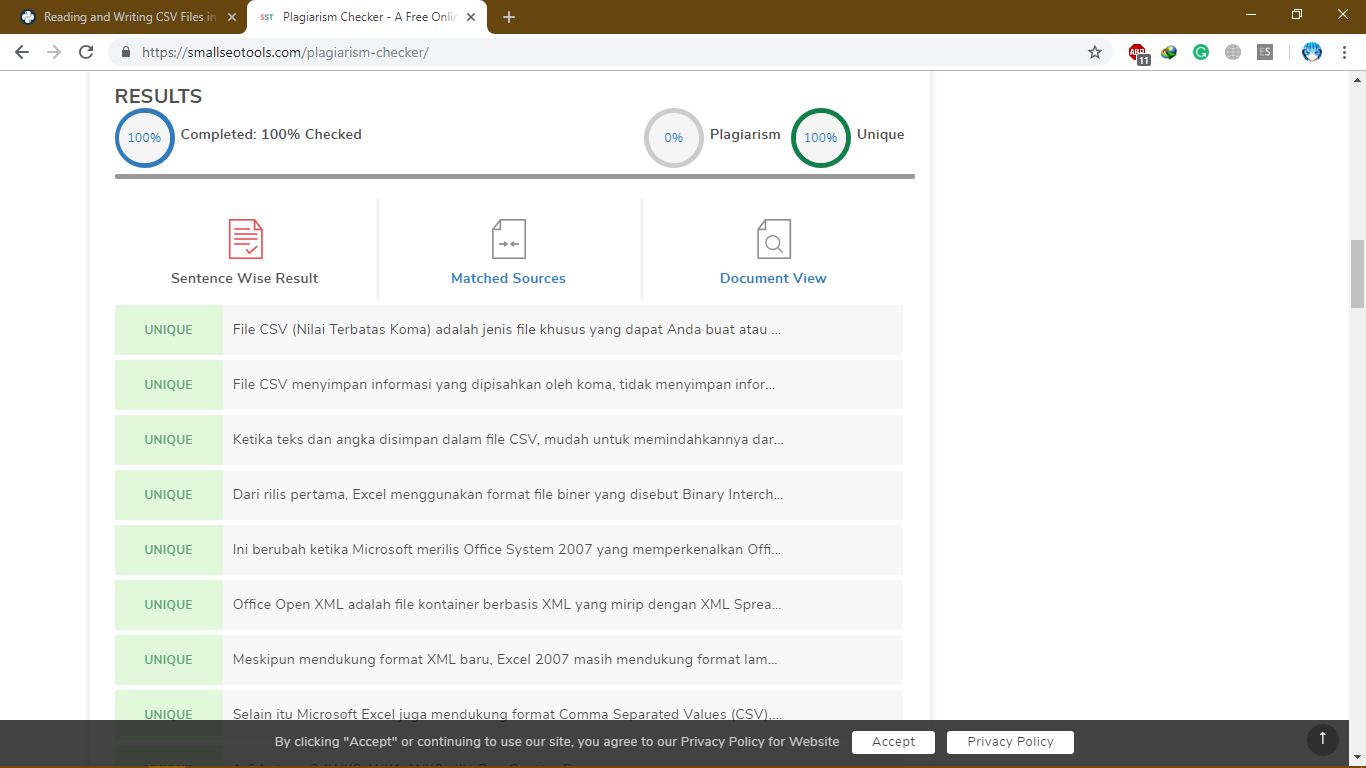
\includegraphics[width=10cm]{figures/4/1174027/teori/harunpla.png}
    \caption{SS Bebas Plagiarisme}
    \label{harun}
\end{figure}

\section{Sri Rahayu}
\subsection{Soal 1}
Isi jawaban soal ke-1

Kalau mau dibikin paragrap \textbf{cukup enter aja}, tidak usah pakai \verb|par| dsb

%\subsection{Soal 2}
%Isi jawaban soal ke-2

%\subsection{Soal 3}
%Isi jawaban soal ke-3

\section{Doli Jonviter}
\subsection{Soal 1}
Isi jawaban soal ke-1

Kalau mau dibikin paragrap \textbf{cukup enter aja}, tidak usah pakai \verb|par| dsb

%\subsection{Soal 2}
%Isi jawaban soal ke-2

%\subsection{Soal 3}
%Isi jawaban soal ke-3

\section{Rahmatul Ridha}
\subsection{Soal 1}
Isi jawaban soal ke-1

Kalau mau dibikin paragrap \textbf{cukup enter aja}, tidak usah pakai \verb|par| dsb

%\subsection{Soal 2}
%Isi jawaban soal ke-2

%\subsection{Soal 3}
%Isi jawaban soal ke-3

\section{Tomy Prawoto}
\subsection{Soal 1}
Isi jawaban soal ke-1

Kalau mau dibikin paragrap \textbf{cukup enter aja}, tidak usah pakai \verb|par| dsb

%\subsection{Soal 2}
%Isi jawaban soal ke-2

%\subsection{Soal 3}
%Isi jawaban soal ke-3
